\chapter{EXPERIMENT RESULTS}
\label{chap:exp}


\section{Experiment Setting}


\begin{table}[hbt]
  \caption{Product data set}
  \label{tab: parameter1}
  \centering
  \begin{tabular}{c|c|c|c|p{5cm}}
    \toprule
    Dataset & d & n & Attributes & Source \\
    \midrule 
    \midrule
    HOTEL  & 4 & 186,637 & hotels-base.com& \parbox{5cm}{No. of stars,\\ No. of rooms, \\No. of facilities, \\Price} \\
    \midrule
    HOUSE  & 6 & 315,063& ipums.org & \parbox{5cm}{Gas, Electricity,\\ Water, Heating,\\ Insurance, Property tax} \\
  \bottomrule
\end{tabular}
\end{table}

\begin{table}[hbt]
  \caption{Experiment parameters and default setting}
  \label{tab: parameter2}
  \centering
  \begin{tabular}{c|c}
    \toprule
    Lemma 3 product samples & 10k, 100K, 1M, {\bfseries 10M}\\
    $card(P)$ &  0, 5000, {\bfseries 10000}, 15000, 20000 \\
    Product dataset & {\bfseries HOTEL}, HOUSE\\
    User data size   & 1000, {\bfseries 5000}, 10000      \\
    User data distribution  & {\bfseries Uniform}, Correlated, Anti-correlated  \\
    $k$ & 5, {\bfseries 10}, 20, 30 \\
    $B$ for HOTEL & 1, {\bfseries 1.25}, 1.5, 2 , 2.5, 3\\
    $B$ for HOUSE & 3, 3.5, 4 ,4.5, 5, 5.5 , 5.7 , 5.9\\
  \bottomrule
\end{tabular}
\end{table}

\begin{figure}[hbt!]
  \centering
  \begin{subfigure}[b]{0.45\linewidth}
    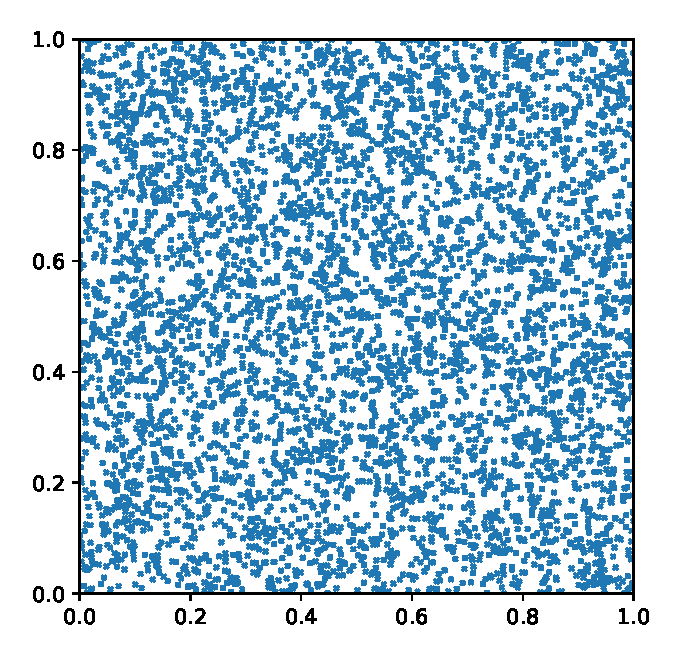
\includegraphics[width=.99\textwidth]{fig_uni}
    \caption{Uniform Distribution Data}
    \label{fig_uni}
  \end{subfigure}
  % %
  % \begin{subfigure}[b]{0.45\linewidth}
  %   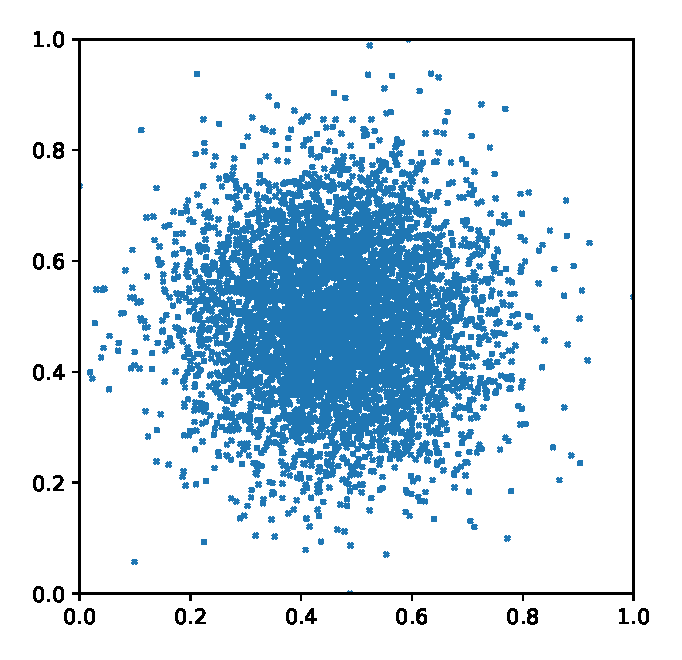
\includegraphics[width=.99\textwidth]{fig_gauss}
  %   \caption{Gaussian Distribution Data}
  %   \label{fig_gauss}
  % \end{subfigure}
  %
  \begin{subfigure}[b]{0.45\linewidth}
    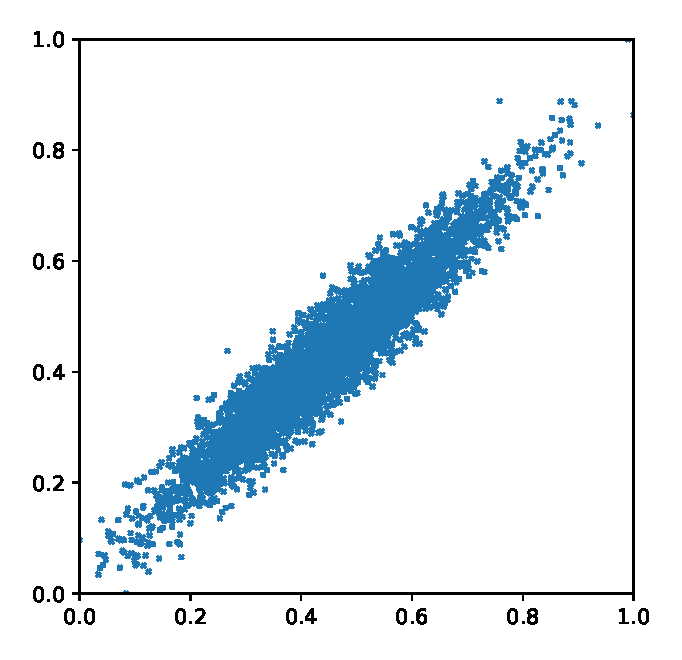
\includegraphics[width=.99\textwidth]{fig_corr}
    \caption{Correlated Distribution Data}
    \label{fig_corr}
  \end{subfigure}
  %
  \begin{subfigure}[b]{0.45\linewidth}
    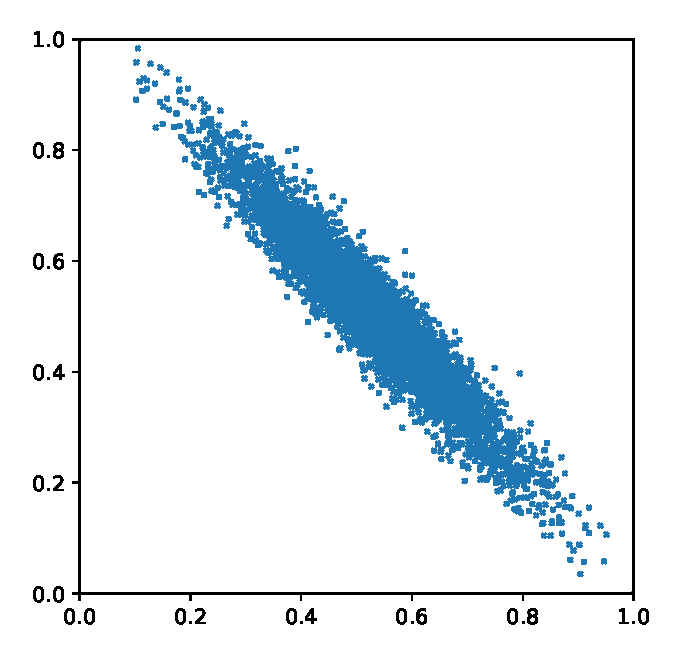
\includegraphics[width=.99\textwidth]{fig_anti}
    \caption{Anti-correlated Distribution Data}
    \label{fig_anti}
  \end{subfigure}
  \caption{Different Distribution Data in 2d}
  \label{data distribution}
\end{figure}

There are 3 kinds of datasets, the product data set $D$, $m=card(D)$; 
the product data set $P$, which uniformly generated by $D$ and so $P\subset D$;
the user data set $W$, all the attributes of data $w\in W$ satisfy $\Sigma w[i]=1$. 
The dimensionality of data is marked as $d$. 
Table \ref{tab: parameter1} shows all the product datasets. 
Table \ref{tab: parameter2} shows the parameters' setting and 
our default setting of them. Figure \ref{data distribution} shows how different
distribution data looks like. For example, if we want to sample products according
to correlated distribution with 2 attributes, then the final generated data will
looks like Figure \ref{fig_corr}.


All codes are implemented by C++; 
the procedure of insertion of $h_i$ needs LP solver and we use $lp\_solve$($http://lpsolve.sourceforge.net/5.5/$)
 to do it and the effciency of $lp\_solve$ has been proved by $kSPR$.  
The running machine is with Intel Xeon Gold 5122 - 3.60 GHz CPU, 128GB DDR4 RAM. 

\section{Effectiveness of Lemmas and Tricks}
In this section, we mainly discuss that how much does each lemma effetively help us
solve $kCRM$. And because there are some parameters within our advance algorithm, 
we would also explore how and why they could influence the efficiency of our algorithm
the way shown in our experiments.


\begin{figure}[ht!]
  \centering
  \begin{subfigure}[b]{0.45\linewidth}
    \includegraphics[width=.99\textwidth]{exp_lemmas1}
    \caption{No. of cells}
    \label{lemmas_on_cell}
  \end{subfigure}
  %
  \begin{subfigure}[b]{0.45\linewidth}
    \includegraphics[width=.99\textwidth]{exp_lemmas2}
    \caption{Time spent in $CellTree$}
    \label{lemmas_on_time}
  \end{subfigure}
  \caption{Effectiveness of Lemmas}
  \label{lemmas}
\end{figure}

Firstly, we would show a global view of each lemmas as in Figure \ref{lemmas}.
-L1 means for advance solution, we apply $C(p)\leq B$ instead of $C(p)=B$ and 
the other optimization will be remained. For -L2, it will take account with those 
users $w_i$ such that $w_i\cdot p=S_{ik}$ doesn't intersect with $C(p)=B$. 
For -L3, it won't generate any lower bound of optimal solution or anything related
to pruning number $\alpha$ and it will just do insertion in $CellTree$ no matter how 
many negative spaces the nodes in. For -L4, it will randomly insert users into $CellTree$.
The default running means, we will
\begin{itemize}
  \item only consider $C(p)=B$
  \item remove unrelated users respecting to $C(p)=B$
  \item sample new product on $C(p)=B$, get lower bound of optimal solution and 
  then use $\alpha$ to prune nodes in $CellTree$.
  \item based on the less likely to be one of the covered users of optimal solution to insert 
  users so as to earlier prune them. 
\end{itemize}


As shown in Figure \ref{lemmas_on_cell}, because Lemma 1 tells that we only take account 
$C(p)=B$, which means we reduce most of the candidate space and reduce problem from 
$d$ dimension to $d-1$ dimension, it will improve our approach by hundreds of times of cells and running time. 
For the other lemmas, it also improves our algorithm by dozens of times.


\begin{figure}[ht!]
  \centering
  \begin{subfigure}[b]{0.45\linewidth}
    \includegraphics[width=.99\textwidth]{exp_L1_0}
    \caption{No. of cells}
    \label{exp_L1_0}
  \end{subfigure}
  %
  \begin{subfigure}[b]{0.45\linewidth}
    \includegraphics[width=.99\textwidth]{exp_L1_1}
    \caption{Time spent in $CellTree$}
    \label{exp_L1_1}
  \end{subfigure}
  \caption{Effectiveness of Lemma 1}
  \label{exp_L1}
\end{figure}

\begin{figure}[ht!]
  \centering
  \begin{subfigure}[b]{0.45\linewidth}
    \includegraphics[width=.99\textwidth]{exp_L2}
    \caption{No. of cells}
    \label{exp_L2_in}
  \end{subfigure}
  \caption{Effectiveness of Lemma 2}
  \label{exp_L2}
\end{figure}

\begin{figure}[ht!]
  \centering
  \begin{subfigure}[b]{0.45\linewidth}
    \includegraphics[width=.99\textwidth]{exp_L3_0}
    \caption{No. of cells}
    \label{exp_L3_0}
  \end{subfigure}
  %
  \begin{subfigure}[b]{0.45\linewidth}
    \includegraphics[width=.99\textwidth]{exp_L3_1}
    \caption{Time spent in $CellTree$}
    \label{exp_L3_1}
  \end{subfigure}
  \caption{Effectiveness of Lemma 3}
  \label{exp_L3}
\end{figure}

\begin{figure}[ht!]
  \centering
  \begin{subfigure}[b]{0.45\linewidth}
    \includegraphics[width=.99\textwidth]{exp_L4_0}
    \caption{No. of cells}
    \label{exp_L4_0}
  \end{subfigure}
  %
  \begin{subfigure}[b]{0.45\linewidth}
    \includegraphics[width=.99\textwidth]{exp_L4_1}
    \caption{Time spent in $CellTree$}
    \label{exp_L4_1}
  \end{subfigure}
  \caption{Effectiveness of Lemma 4}
  \label{exp_L4}
\end{figure}

\begin{figure}[ht!]
  \centering
  \begin{subfigure}[b]{0.45\linewidth}
    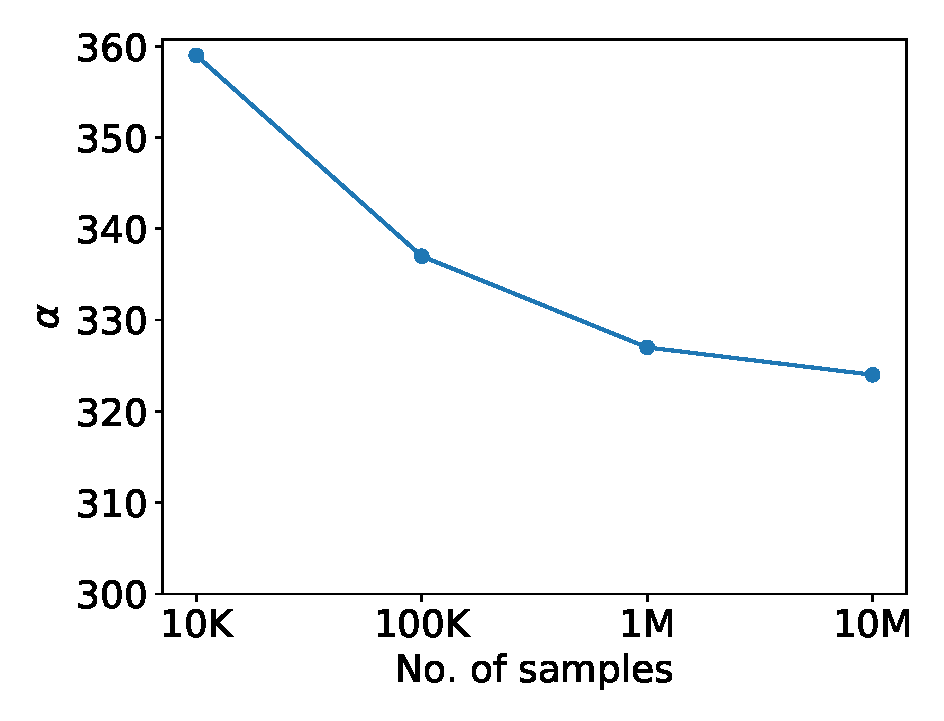
\includegraphics[width=.99\textwidth]{exp_sampleCnt0}
    \caption{pruning number $\alpha$}
    \label{newpdtcnt_on_alpha}
  \end{subfigure}
  %
  \begin{subfigure}[b]{0.45\linewidth}
    \includegraphics[width=.99\textwidth]{exp_sampleCnt1}
    \caption{No. of cells}
    \label{newpdtcnt_on_cell}
  \end{subfigure}
  %
  \begin{subfigure}[b]{0.45\linewidth}
    \includegraphics[width=.99\textwidth]{exp_sampleCnt2}
    \caption{Time spent in $CellTree$}
    \label{newpdtcnt_on_time}
  \end{subfigure}
  \caption{Effect of No. of newly sampled products}
  \label{lemma3_cnt}
\end{figure}

For each of lemmas, we make some experiments for details of how efficient they are.
In Figure \ref{exp_L1}, $-L1$ means when the situation without applying Lemma 1 but 
keeping the other lemmas work. With the change of cardinality of user dataset $W$,
$CellTree$'s cell number and running time grow fast for $-L1$ while grow more slower
for $L1$. In Figure \ref{exp_L2}, we skip the previous step that remove the users 
that covered by $P$ and clearly see that the number users, whose $w_i\cdot p=B$ 
would intersect constraint $C(p)=B$, grows linearly with cardinality of $W$. 
In Figure \ref{exp_L3}, we applying other lemmas but without Lemma 3, which 
using lower bound of optimal solution to prune tree cells of $CellTree$, comparing
applying Lemma 3 shows that Lemma 3 help us save space and time efficiently. Figure
\ref{exp_L4} also shows the effectiveness of Lemma 4 which changes the insertion order of
users to $CellTree$ in order to earlier prune the nodes that unlikely to be the
ancestor cell of optimal solution nodes.


In Lemma 3 we say that we would sample new products on $C(p)=B$ to get pruning number and 
next we will show the cardinality of newly generated new products influences our algorithm.
 The sampling time is negligible
for time in $CellTree$ insertion and we won't discuss the time spent by sampling in this section.
As shown in Figure \ref{newpdtcnt_on_alpha}, $\alpha$ slowly decreases with the increment of samples. 
We can also see from Figure \ref{newpdtcnt_on_cell} and Figure \ref{newpdtcnt_on_time} though
the change of $\alpha$ is small, but it makes a huge impact on resulting cells number in 
$CellTree$. This can explained by our algorithm's time complexity, $O(n^d)$, which means a 
litter change of users improves response time huge. 



\section{Influence of Inputs}
In this section, we would show the compact of input parameters to our algorithm. 

\begin{figure}[ht!]
  \centering
  \begin{subfigure}[b]{0.45\linewidth}
    \includegraphics[width=.99\textwidth]{exp_cardW0}
    \caption{Processed users in $CellTree$}
    \label{exp_cardW0}
  \end{subfigure}
  %
  \begin{subfigure}[b]{0.45\linewidth}
    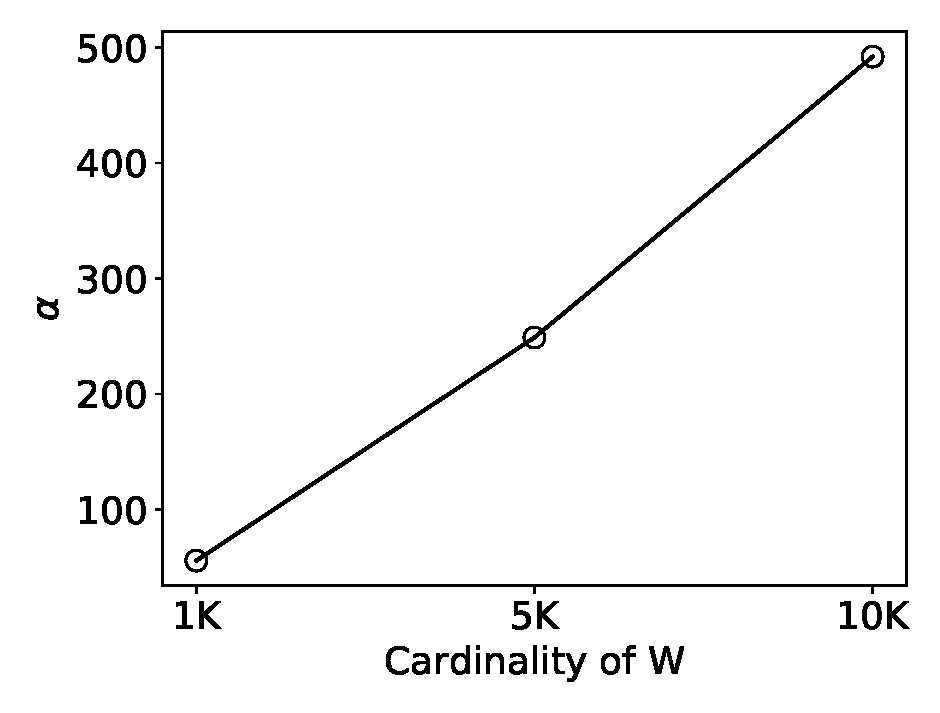
\includegraphics[width=.99\textwidth]{exp_cardW1}
    \caption{Pruning number $\alpha$}
    \label{exp_cardW1}
  \end{subfigure}
  %
  \begin{subfigure}[b]{0.45\linewidth}
    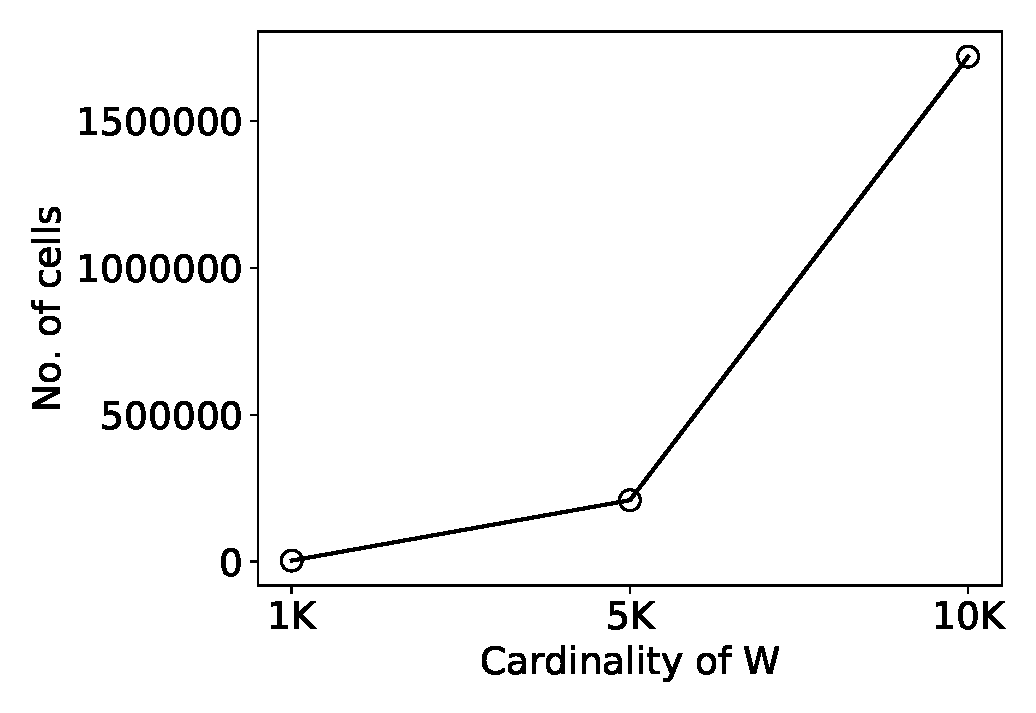
\includegraphics[width=.99\textwidth]{exp_cardW2}
    \caption{No. of cells}
    \label{exp_cardW2}
  \end{subfigure}
  %
  \begin{subfigure}[b]{0.45\linewidth}
    \includegraphics[width=.99\textwidth]{exp_cardW3}
    \caption{Time spent in $CellTree$}
    \label{exp_cardW3}
  \end{subfigure}
  \caption{Effect of cardinality of user dataset $W$}
  \label{cardW}
\end{figure}

Since the time complexity is $O(n^d)$, we can see from Figure \ref{cardW} that the users 
remain to be inserted in $CellTree$ grow linearly while the resulting cells and response 
time growing exponentially. 


\begin{figure}[hbt!]
  \centering
  \includegraphics[width=.5\linewidth]{exp_lemmas0}
  \caption{Effect of $card(P)$ on user uncovered by $P$}
  \label{p_on_user}
\end{figure}
Product dataset $P$ will influence the efficiency of solving problems because in some
extreme condition, or unluckily $P$ only covers a few users; but sometime, $P$ will covers 
most of users. To complete the experiment of explore the global view impact of 
cardinality of $P$, we run 20 times sampling different $P$ for each attribute as shown in 
Figure \ref{p_on_user}. The original user data sizes are all 5000 and are the same. The y
axis means how many users is left that uncovered by $P$. We can see from Figure 
\ref{p_on_user} such that with the increment of cardinality of $P$, uncovered 
users number decreases slower and slower. 



\begin{figure}[ht!]
  \centering
  \begin{subfigure}[b]{0.45\linewidth}
    \includegraphics[width=.99\textwidth]{exp_topk0}
    \caption{User uncovered by $P$}
    \label{k_change_user_cnt}
  \end{subfigure}
  %
  \begin{subfigure}[b]{0.45\linewidth}
    \includegraphics[width=.99\textwidth]{exp_topk1}
    \caption{Time spent in $CellTree$}
    \label{k_change_time}
  \end{subfigure}
  \caption{Effect of k (HOTEL)}
  \label{k_effect}
\end{figure}

Now we explore the impact of $k$. Our problem is to find a new product that rank as more as possible 
users' top $k$ as possible, and we have a prerequisite such that product dataset $P$ already 
covers a part of the users. With the increasing $k$, unchanged product dataset and 
user dataset, the products in dataset $P$ are to cover more users easily because the 
the threshold to be a user's top-$k$ is lowering down. With $P$ covering more users, no matter 
which of the lemmas
we propose or the baseline $CellTree$ approach will all greatly benefit from the reducing 
users. We show the experiment in Figure \ref{k_effect}. The y axis of Figure 
\ref{k_change_user_cnt} means the users number that we need to handle after removing 
the users that covered by $P$. We can see that user dataset with size 1000, 5000 or 10000, their 
uncovered users decrease exponentially with the change of k. And because of the decreasing
uncovered users, our response time also decreases exponentially.

\section{Effect of Product Dataset Distribution and B}

\begin{figure}[ht!]
  \centering
  \begin{subfigure}[b]{0.45\linewidth}
    \includegraphics[width=.99\textwidth]{uni2dex0}
    \caption{Products and users covered by $P$}
    \label{cover_uni}
  \end{subfigure}
  %
  \begin{subfigure}[b]{0.45\linewidth}
    \includegraphics[width=.99\textwidth]{uni2dex1}
    \caption{Uniform, B=1.1}
    \label{it_uni_1_1}
  \end{subfigure}
  %
  \begin{subfigure}[b]{0.45\linewidth}
    \includegraphics[width=.99\textwidth]{uni2dex2}
    \caption{Uniform, B=1.3}
    \label{it_uni_1_3}
  \end{subfigure}
  %      
  \begin{subfigure}[b]{0.45\linewidth}
    \includegraphics[width=.99\textwidth]{uni2dex3}
    \caption{Uniform, B=1.5}
    \label{it_uni_1_5}
  \end{subfigure}
  %
  \begin{subfigure}[b]{0.45\linewidth}
    \includegraphics[width=.99\textwidth]{uni2dex4}
    \caption{Uniform, B=1.7}
    \label{it_uni_1_7}
  \end{subfigure}
  %      
  \begin{subfigure}[b]{0.45\linewidth}
    \includegraphics[width=.99\textwidth]{uni2dex5}
    \caption{Uniform, B=1.9}
    \label{it_uni_1_9}
  \end{subfigure}
  \caption{Effect of $B$ on uniform products}
  \label{uni_2d_demo}
\end{figure}



\begin{figure}[ht!]
  \centering
  \begin{subfigure}[b]{0.45\linewidth}
    \includegraphics[width=.99\textwidth]{corr2dex0}
    \caption{Products and users covered by $P$}
    \label{cover_corr}
  \end{subfigure}
  %
  \begin{subfigure}[b]{0.45\linewidth}
    \includegraphics[width=.99\textwidth]{corr2dex1}
    \caption{Corr, B=1.1}
    \label{it_corr_1_1}
  \end{subfigure}
  %
  \begin{subfigure}[b]{0.45\linewidth}
    \includegraphics[width=.99\textwidth]{corr2dex2}
    \caption{Corr, B=1.3}
    \label{it_corr_1_3}
  \end{subfigure}
  %      
  \begin{subfigure}[b]{0.45\linewidth}
    \includegraphics[width=.99\textwidth]{corr2dex3}
    \caption{Corr, B=1.5}
    \label{it_corr_1_5}
  \end{subfigure}
  %
  \begin{subfigure}[b]{0.45\linewidth}
    \includegraphics[width=.99\textwidth]{corr2dex4}
    \caption{Corr, B=1.7}
    \label{it_corr_1_7}
  \end{subfigure}
  %      
  \begin{subfigure}[b]{0.45\linewidth}
    \includegraphics[width=.99\textwidth]{corr2dex5}
    \caption{Corr, B=1.9}
    \label{it_corr_1_9}
  \end{subfigure}
  \caption{Effect of $B$ on corr products}
  \label{corr_2d_demo}
\end{figure}

\begin{figure}[ht!]
  \centering
  \begin{subfigure}[b]{0.45\linewidth}
    \includegraphics[width=.99\textwidth]{anti2dex0}
    \caption{Products and users covered by $P$}
    \label{cover_anti}
  \end{subfigure}
  %
  \begin{subfigure}[b]{0.45\linewidth}
    \includegraphics[width=.99\textwidth]{anti2dex1}
    \caption{Anti, B=1.1}
    \label{it_anti_1_1}
  \end{subfigure}
  %
  \begin{subfigure}[b]{0.45\linewidth}
    \includegraphics[width=.99\textwidth]{anti2dex2}
    \caption{Anti, B=1.3}
    \label{it_anti_1_3}
  \end{subfigure}
  %      
  \begin{subfigure}[b]{0.45\linewidth}
    \includegraphics[width=.99\textwidth]{anti2dex3}
    \caption{Anti, B=1.5}
    \label{it_anti_1_5}
  \end{subfigure}
  %
  \begin{subfigure}[b]{0.45\linewidth}
    \includegraphics[width=.99\textwidth]{anti2dex4}
    \caption{Anti, B=1.7}
    \label{it_anti_1_7}
  \end{subfigure}
  %      
  \begin{subfigure}[b]{0.45\linewidth}
    \includegraphics[width=.99\textwidth]{anti2dex5}
    \caption{Anti, B=1.9}
    \label{it_anti_1_9}
  \end{subfigure}
  \caption{Effect of $B$ on anti products}
  \label{anti_2d_demo}
\end{figure}

To straight forward presents our algorithm and shows the interesting finding in
experiments, we use a 2d experiment and visualize it as in Figure 
\ref{uni_2d_demo}, \ref{corr_2d_demo} and \ref{anti_2d_demo}.

First of all, the users are all generated uniformly from $w[1]+w[2]=1$.

To explain Figure \ref{uni_2d_demo}, \ref{corr_2d_demo} and \ref{anti_2d_demo}, we
take \ref{cover_uni} as an example, this figure is drawn in product space. 
Product dataset $D$ consists with the grey, blue and red points
; product dataset $P$ consists with the blue and red points; the red points are the points that 
each of them at least covers one user.  Specially, 
we have to expand the size of red points to clearly show them. We can see the red points
of Figure \ref{cover_uni} at about $(0.9, 0.9)$ and $(0.95, 0.8)$.
The lines are all $w_i\dot p=S_{ik}$. The blue lines mean the corresponding $w_i\dot p=S_{ik}$ of users 
that covered by $P$ and the rest users' halfspaces are orange lines. From Figure 
\ref{it_uni_1_1} to Figure \ref{it_uni_1_9}, the bold black line means 
the constraint $\Sigma_{i=1}^d p[i]\leq B$ when $B$ equals 1.1, 1.3, 1.5, 1.7, 1.9 respectively.
The orange lines mean the $w_i\dot p=S_{ik}$ that intersects with constraint and the blues aren't
intersect with constraint. 

In Figure \ref{cover_uni}, because the distribution of products is uniform so 
for each user weight vector $w_i$, there is a proper product $p_{wi}$ nearby the extend of
$w_i$ ranks top-$k$ for it. And because the halfspace $w_i\cdot p=S_{ik}$ getting through the point $p_{wi}$,
so the lower bounds of $w_i\dot p=S_{ik}$ makes a smooth curve along $p[2]=1$ and
$p[1]=1$. From Figure \ref{it_uni_1_1} to Figure \ref{it_uni_1_9}, the number of the halfspaces
that intersect with constraint increases with the increasing $B$ because more and more 
products become some of the users' top-$k$ and so as will more halfspaces be there.


In Figure \ref{cover_corr}, the red point is around $(0.9, 0.9)$. In correlated 
distribution products as shown in \ref{cover_corr}, almost all the products that 
rank $k$ for users are at the location that is closed to $(1, 1)$. Because the 
halfspaces will get through the points that rank exactly $k$ and
products ranking $k$ are almost the same or very closed to each other, it seems all
halfspaces intersect at one point. Be careful that they aren't intersect at exact
one point and it looks so just because of the size of figure we can show. The halfspaces
that intersect with constraint will gradually increase and at a special B decrease
suddenly as we can see from Figure \ref{it_corr_1_1} to Figure \ref{it_corr_1_9}.

In Figure \ref{cover_anti}, the red points are about at $(0.1, 0.95)$, $(0.3, 0.8)$, $(0.8, 0.3)$.
The products that exactly rank $k$ for users concentrate on $(0.2, 0.9)$ and $(0.9, 0.2)$.
This could be explained by the Lemma 4 of $k-hit query$, which says that for any 
weight vector $w$ if only a point $p_ix$ inside the convex hull made by 
$P_i=\{p_i1, p_i2, ..., p_{i(x-1)}\}$, then there must be a point in $P_i$
such that its dot product with $w$ is higher than $p_ix$'s. 
For our case of anti-correlated distribution products, most of products are between
the points nearby $(0, 1)$ and $(1, 0)$ which means for any weight vector, its top-$k$
is nearby $(0, 1)$ or $(1,0)$ when $k$ is small and $card(D)$ is also large. Therefore,
in Figure \ref{anti_2d_demo} we can see most of halfspaces getting through $(0.2, 0.9)$ and $(0.9, 0.2)$
which is closed to $(0,1)$ or $(1, 0)$. With the increasing of $B$, the number of 
halfspaces that 
intersect with constraint suddenly increases and then gradually decreases. 


In Figure \ref{uni_2d_demo}, \ref{corr_2d_demo} and \ref{anti_2d_demo}, we show the process of our
algorithm to solve $kCRM$. Firstly, remove the users that covered by $P$. Remove the 
halfspaces $w_i\cdot p=S_{ik}$ that doesn't intersect with constraint. Change
the insertion order of halfspaces by some heuristic. Use $CellTree$
proposed in $kSPR$ to find the region that cover the most of the rest of users.
During the process in $CellTree$, prune the tree nodes with lower bound of optimal
solution.



\begin{figure}[hbt!]
  \centering
  \begin{subfigure}[b]{0.8\linewidth}
    \includegraphics[width=.99\textwidth]{inters_B}
  \end{subfigure}
  \caption{No. of halfspaces intersect with constraint}
  \label{inters_B}
\end{figure}

Figure \ref{inters_B} shows the exact changes of halfspaces. 

For uniform generated
products, intersect halfspaces increases gradually. If the new proposed product wants 
to cover as more user as possible, its attributes should balance and all with high
values. And if the new product is already a top-$k$ option for some users, it is 
hard for it to cover more because each aspect of it is already high and the cost of
develop such product is too high to afford or too hard to realize. But still, we
could introduce the product that only satisfies some kind of users. For example,
to cover users that care more about $p[1]$, we can introduce the new product as
$p=(1, 0.5)$ under the constraint $p[1]+p[2]\leq 1.5$. 

For correlated generated products,
intersect halfspace increases gradually and then suddenly decrease. For this kind of
product distribution, it is also recommended to introduce new products that with 
high value in some attribute. It is easy for correlated products to introduce a new product
that cover all of the users since there are already existing several products 
cover all of users but for uniformly products it is not likely to find product that 
cover all users.


For anti-correlated
generated products, intersect halfspaces firstly increases for a short time and then
gradually decreases. In real world, most of the product datasets are based on this 
distribution, such as $HOTEL$ and $HOUSE$ data proposed in this paper.  For each
attribute, there is a certain value that if the product's corresponding attribute
exceeds it then this product will cover a kind of users. To cover different kinds 
of users, the new product has to balance each attribute. Because in real world
the users that favor in each attribute are unbalance. For example, there are more 
users prefer
computers with powerful computation ability than with large memory. Consider the case
$P=\emptyset$, to cover more users the new product just needs to with high value
in the attribute that considered more important by most users. When $P\neq \emptyset$, 
as we can see from Figure \ref{cover_anti}, to covered all of the rest user(the orange lines), we need
to introduce products such as $\{(0.1, 0.95), (0.95, 0.1)\}$. To covered them by a single
product, we need a product for example no worse than $(0.9, 0.7)$. But in realistic, 
the option decision maker isn't likely to introduce such single product under the 
limitation of technology, money and other factors. The best strategy is to firstly 
introduce product $(0.95,0.1)$ and then is $(0.1, 0.95)$. It is hard to cover
all the users and company should take good evaluation of market so as to step by
step make more profits.


 
